\documentclass[norsk,a4paper,12pt]{article}
% if you want a single-column, remove reprint

% allows special characters (including æøå)
\usepackage[utf8]{inputenc}
\usepackage [norsk]{babel} %if you write norwegian
%\usepackage[english]{babel}  %if you write english


\usepackage{physics,amssymb}  % mathematical symbols (physics imports amsmath)
\usepackage{graphicx}         % include graphics such as plots
\usepackage{xcolor}           % set colors
\usepackage{hyperref}         % automagic cross-referencing (this is GODLIKE)
\usepackage{tikz}             % draw figures manually
\usepackage{listings}         % display code
\usepackage{subfigure}        % imports a lot of cool and useful figure commands
\usepackage{float}			  % force placement of tables and figures
\usepackage{amsmath}
\usepackage{minted} %code

\hypersetup{ % this is just my personal choice, feel free to change things
	colorlinks,
	linkcolor={red!50!black},
	citecolor={blue!50!black},
	urlcolor={blue!80!black}}

%% Defines the style of the programming listing
%% This is actually my personal template, go ahead and change stuff if you want
\lstset{ %
	inputpath=,
	backgroundcolor=\color{white!88!black},
	basicstyle={\ttfamily\scriptsize},
	commentstyle=\color{magenta},
	language=Python,
	morekeywords={True,False},
	tabsize=4,
	stringstyle=\color{green!55!black},
	frame=single,
	keywordstyle=\color{blue},
	showstringspaces=false,
	columns=fullflexible,
	keepspaces=true}

\title{FYS3110 - Oblig 3 - Karl Henrik Fredly}

\begin{document}
	
	\maketitle
	
\section*{Problem 3.7(X)}

	\subsection*{a)}
		\begin{equation}
		\begin{aligned}
		(\comm{\hat{A}}{\hat{B}})^\dagger &= (\hat{A}\hat{B} - \hat{B}\hat{A})^\dagger = (\hat{A}\hat{B})^\dagger - \hat{A}^\dagger\hat{B}^\dagger = \hat{A}\hat{B} - \hat{A}\hat{B} = 0 \\
		&\Rightarrow \comm{\hat{A}}{\hat{B}} = 0
		\end{aligned}
		\end{equation}
		Siden $\hat{A}\hat{B}$ er hermitisk og komplekskonjugering kun sender 0 på 0.
		
	\subsection*{b)}
		Ressonomentet i a) gjelder helt likt for $\hat{A}$ og $\hat{C}$. Siden $\hat{A}$, $\hat{B}$ og $\hat{C}$ alle er hermitiske og kommuterer med $\hat{A}$ deler de egentilstander. Siden spekteret til $\hat{A}$ ikke er degenerert kan vi skrive $\hat{B}$ og $\hat{C}$ uttrykt ved egenverdidekomposisjon, altså egentilstandene i ortonormale matriser og en diagonal matrise med egenverdiene sine slik at vi får:
		\begin{equation}
		\begin{aligned}
		(\comm{B}{C})^\dagger &= BC - CB = UD_BU^\dagger UD_CU^\dagger - UD_CU^\dagger UD_BD^\dagger \\
		&= UD_B D_CU^\dagger - UD_CD_BU^\dagger = UD_B D_CU^\dagger - UD_BD_CU^\dagger = 0
		\end{aligned}
		\end{equation}
		Siden diagonale matriser alltid kommuterer. B og C deler egentilstander, så $\psi_2$ er en egentilstand til C med egenverdi $\lambda_{C2}$ og vi får:
		\begin{equation}
		\begin{aligned}
		\bra{\psi_1}\hat{C}\ket{\psi_2} = \bra{\psi_1}\lambda_{C2}\ket{\psi_2} = \lambda_{C2}\bra{\psi_1}\ket{\psi_2} = 0
		\end{aligned}
		\end{equation}
		
\section*{Problem 3.8(H)}

	\subsection*{a)}
		Finner hvor $\hat{H}$ sender standardbasisvektorene, og setter det som kolonnene i $\hat{H}$.
		\begin{equation*}
		\begin{aligned}
		\mathbf{\hat{H}} = \begin{bmatrix}
		-V & -g & 0 & 0 \\
		-g & 0 & -g & 0 \\
		0 & -g & 0 & -g \\
		0 & 0 & -g & 0 \\
		\end{bmatrix}
		\end{aligned}
		\end{equation*}
		
	\subsection*{b)}
		Finner hvor $\hat{X}$ sender standardbasisvektorene, og setter det som kolonnene i $\hat{X}$.
		\begin{equation*}
		\begin{aligned}
		\mathbf{\hat{H}} = \begin{bmatrix}
		0 & 0 & 0 & 0 \\
		0 & 1 & 0 & 0 \\
		0 & 0 & 2 & 0 \\
		0 & 0 & 0 & 3 \\
		\end{bmatrix}
		\end{aligned}
		\end{equation*}
		
	\subsection*{c)}
	Liten vegg med kode:
	\begin{minted}[mathescape, linenos]{python}
import numpy as np
import matplotlib.pyplot as plt

V = 5
g = 1

L = 25
#Hamiltonian
H = np.zeros((L, L))
H[0, 0] = -V
H[0, 1] = -g
for i in range(1, L-1):
    H[i, i-1] = -g
    H[i, i+1] = -g
H[L-1, L-2] = -g
#X
X = np.zeros((L, L))
for i in range(L):
    X[i, i] = i
#Gjør det enkelt
eigVals = np.linalg.eig(H)[0]
eigVecs = np.linalg.eig(H)[1]
print(eigVals[0])
plt.hlines(eigVals, 0, 1)
plt.xticks([])
plt.savefig("energylevel")
plt.show()
	\end{minted}
	Den laveste energien er -5.2.
	\begin{figure}[H]
		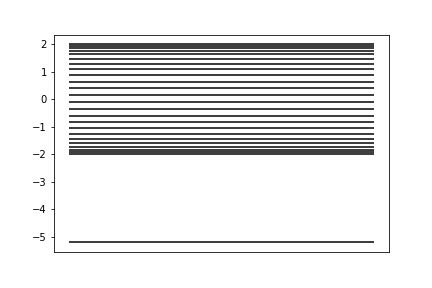
\includegraphics[width=90mm]{../energylevel.png}
		\caption{Energinivåene.}
		\label{fig:energylevel}
	\end{figure}
	
	\subsection*{d)}
	\begin{minted}[mathescape, linenos]{python}
GS = eigVecs[:,0]
print(GS[0]**2)
print(eigVecs[:,0][1]**2)
	\end{minted}
	Sannsynligheten for å finne elektronet på atom 0 er 0.96, og sannsynligheten for å finne elektroner på atom 1 er 0.0384.
	
	\subsection*{e)}
	\begin{minted}[mathescape, linenos]{python}
print(np.inner(np.conj(GS), X @ GS))
	\end{minted}
	Forventningsverdien til posisjonen i grunntilstanden er 0.0417, altså veldig nært 0.
	
	\subsection*{f)}
	Finner $\ket{0}$ som en lineærkombinasjon av energiegentilstandene, og finner tidsutviklingen ved å gi hver komponent i lineærkombinasjonen sin egen eksponential gitt ved egenverdien for energi.
	\begin{minted}[mathescape, linenos]{python}
v0 = np.zeros(L); v0[0] = 1
coeffs = np.linalg.solve(eigVecs, v0)
hbar = 1
def prob0(t):
    total = 0
    for i in range(L):
        total += eigVecs[:,i][0] * coeffs[i] * np.exp(-1j / hbar * eigVals[i] * t)
    return np.abs(total)**2
    
t = np.linspace(0, 100, 1000)
plt.plot(t, prob0(t))
plt.savefig("tidsutvikling")
plt.show()
	\end{minted}
	\begin{figure}[H]
		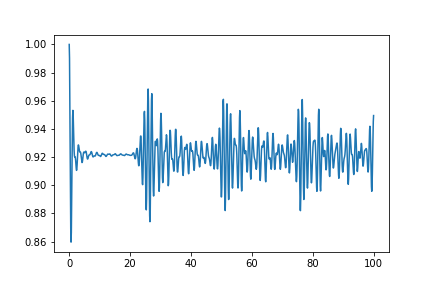
\includegraphics[width=90mm]{../tidsutvikling.png}
		\caption{Tidsutviklingen fra måling av elektronet i $\ket{0}$.}
	\end{figure}

	\subsection*{g)}
	Ved omtrent t=23$\hbar$ begynner $P_0(t)$ å oscillere mye mer. En mulighet kan være at en bølge som spredte seg ved starten av tidsutviklingen til de andre posisjonene begynner å komme tilbake.
	
\section*{Problem 3.9(H)}

	\subsection*{a)}
	\begin{equation*}
	\begin{aligned}
	\mathbf{\hat{H}^\dagger} = \begin{bmatrix}
	1 & (\frac{-i}{2})^* & 0 \\
	(\frac{i}{2})^* & 1 & 0 \\
	0 & 0 & \frac{1}{2} \\
	\end{bmatrix}
	= \begin{bmatrix}
	1 & \frac{i}{2} & 0 \\
	\frac{-i}{2} & 1 & 0 \\
	0 & 0 & \frac{1}{2} \\
	\end{bmatrix} = \mathbf{\hat{H}}
	\end{aligned}
	\end{equation*}
	
	\subsection*{b)}
	\begin{equation*}
	\begin{aligned}
	\mathbf{\hat{H}\ket{1}} = \begin{bmatrix}
	1 & \frac{i}{2} & 0 \\
	\frac{-i}{2} & 1 & 0 \\
	0 & 0 & \frac{1}{2} \\
	\end{bmatrix} \frac{1}{\sqrt{2}} \begin{bmatrix}
	i \\
	1 \\
	0 \\
	\end{bmatrix} = \frac{1}{\sqrt{2}} \begin{bmatrix}
	i + \frac{i}{2}\\
	\frac{-i^2}{2} + 1 \\
	0 \\
	\end{bmatrix} = \frac{1}{\sqrt{2}} \begin{bmatrix}
	\frac{3i}{2}\\
	\frac{3}{2} \\
	0 \\
	\end{bmatrix} = \frac{3}{2} \ket{1}
	\end{aligned}
	\end{equation*}
	
	\begin{equation*}
	\begin{aligned}
	\mathbf{\hat{H}\ket{2}} = \begin{bmatrix}
	1 & \frac{i}{2} & 0 \\
	\frac{-i}{2} & 1 & 0 \\
	0 & 0 & \frac{1}{2} \\
	\end{bmatrix} \begin{bmatrix}
	0 \\
	0 \\
	1 \\
	\end{bmatrix} = \frac{1}{\sqrt{2}} \begin{bmatrix}
	0\\
	0 \\
	\frac{1}{2} \\
	\end{bmatrix} =  \frac{1}{2} \ket{2}
	\end{aligned}
	\end{equation*}
	
	\begin{equation*}
	\begin{aligned}
	\mathbf{\hat{H}\ket{3}} = \begin{bmatrix}
	1 & \frac{i}{2} & 0 \\
	\frac{-i}{2} & 1 & 0 \\
	0 & 0 & \frac{1}{2} \\
	\end{bmatrix} \frac{1}{\sqrt{3}} \begin{bmatrix}
	-i \\
	1 \\
	-1 \\
	\end{bmatrix} = \frac{1}{\sqrt{3}} \begin{bmatrix}
	-i + \frac{i}{2} \\
	\frac{i^2}{2} + 1 \\
	\frac{-1}{2} \\
	\end{bmatrix} = \frac{1}{\sqrt{3}} \begin{bmatrix}
	\frac{-i}{2}\\
	\frac{1}{2} \\
	\frac{-1}{2} \\
	\end{bmatrix} = \frac{1}{2} \ket{3}
	\end{aligned}
	\end{equation*}

	\subsection*{c)}
	Regnet ut med python:
	\begin{minted}[mathescape, linenos]{python}
H9 = np.array([
    [1, 0.5j, 0],
    [-0.5j, 1, 0],
    [0, 0, 0.5]
])
v1 = 1/2**0.5 * np.array([1j, 1, 0])
v2 = np.array([0, 0, 1])
v3 = 1/3**0.5 * np.array([-1j, 1, -1])
for i in [v1, v2, v3]:
    for j in [v1, v2, v3]:
        print(np.inner(np.conj(i), H9 @ j))
for i in [1, 2, 3]: #printer tilsvarende indekser for å være sikker på plasseringer
    for j in [1, 2, 3]:
        print(i , j)
	\end{minted}
	
	\begin{equation*}
	\begin{aligned}
	\mathbf{\hat{H}} = \begin{bmatrix}
	1.5 & 0 & 0 \\
	0 & 0.5 & -0.288 \\
	0 & -0.289 & 0.5 \\
	\end{bmatrix}
	\end{aligned}
	\end{equation*}
	Matrisen er ikke diagonal.
	
	\subsection*{d)}
	
	Ser at $\bra{2}$ og $\bra{3}$ ikke er ortogonale. Finner projeksjonen av $\bra{2}$ på $\bra{3}$:
	\begin{equation*}
	\begin{aligned}
	\bra{3}\ket{2} \ket{2} = -\frac{1}{\sqrt{3}} \ket{2}
	\end{aligned}
	\end{equation*}
	Vi definerer da en ny egenket:
	\begin{equation*}
	\ket{3'} = \ket{3} - \bra{3}\ket{2} \ket{2} = \frac{1}{\sqrt{3}} \begin{bmatrix}
	-i \\
	1 \\
	0 \\
	\end{bmatrix}
	\end{equation*}
	Normerer og får istedet en faktor $\frac{1}{\sqrt{2}}$ foran. Vi får:
	\begin{minted}[mathescape, linenos]{python}
v3 = 1/2**0.5 * np.array([-1j, 1, 0])
for i in [v1, v2, v3]:
    for j in [v1, v2, v3]:
        print(np.inner(np.conj(i), H9 @ j))
	\end{minted}
	\begin{equation*}
	\begin{aligned}
	\mathbf{\hat{H}} = \begin{bmatrix}
	1.5 & 0 & 0 \\
	0 & 0.5 & 0 \\
	0 & 0 & 0.5 \\
	\end{bmatrix}
	\end{aligned}
	\end{equation*}
	$\hat{H}$ blir diagonal med egenverdiene i riktig rekkefølge langs diagonalen som vi forventer.
	
\section*{Problem 3.10(H)}

	Vi ser at alle $\ket{\gamma_n}$ er egenvektorer med egenverdi 0. Det gjenstår å se etter egenvektorer i rommet spent ut av $\ket{\psi}$ og $\ket{\phi}$. Vi kan skrive en lineærkombinasjon av disse som $\ket{\lambda} = a\ket{\psi} + \ket{\phi}$. Setter opp egenverdiligningen for $\ket{\lambda}$ og ser hvilke a som gir en egenvektor.
	
	\begin{equation*}
	\begin{aligned}
	&\hat{H}\ket{\lambda} = \hat{H}(a\ket{\psi} + \ket{\phi}) = g^*\ket{\psi} + ag\ket{\phi}) \\
	&\Rightarrow \frac{a}{g^*} = \frac{1}{ag} \Rightarrow a^2 = \frac{g^*}{g} \Rightarrow a = \pm \sqrt{\frac{g^*}{g}}
	\end{aligned}
	\end{equation*}
	Vi finner egenverdiene ved å sette inn a:
	\begin{equation*}
	\begin{aligned}
	\hat{H}(\sqrt{\frac{g^*}{g}}\ket{\psi} + \ket{\phi}) = g^*\ket{\psi} + \sqrt{\frac{g^*}{g}}g\ket{\phi}) = \sqrt{gg^*}(\sqrt{\frac{g^*}{g}}\ket{\psi} + \ket{\phi})
	\end{aligned}
	\end{equation*}
	\begin{equation*}
	\begin{aligned}
	\hat{H}(-\sqrt{\frac{g^*}{g}}\ket{\psi} + \ket{\phi}) = g^*\ket{\psi} - \sqrt{\frac{g^*}{g}}g\ket{\phi}) = -\sqrt{gg^*}(-\sqrt{\frac{g^*}{g}}\ket{\psi} + \ket{\phi})
	\end{aligned}
	\end{equation*}
	$\hat{H}$ har altså også egentilstand $(\sqrt{\frac{g^*}{g}}\ket{\psi} + \ket{\phi})$ med egenverdi $\sqrt{gg^*}$ og egentilstand $(-\sqrt{\frac{g^*}{g}}\ket{\psi} + \ket{\phi})$ med egenverdi $-\sqrt{gg^*}$.
	
\end{document}